\chapter{Methodology for Estimating Fatigue Life of Dynamic Power Cable }
\label{chap:estimation}
In this section a brief overview of the algorithm for estimating the fatigue life of dynamic power cable will be presented. 
\section{Global Analysis}
First, the global analysis was carried out. The global model described in Section \ref{sec:globmod} was used and the 176 sea states presented in Figure \ref{fig:scatn} was analyzed for 1 hour each, for each of the three weather conditions described in Section \ref{sec:current}. The  tension in the upper element of the cable, and the displacement of the dummy node on the vessel, the first and second node on the cable in x, y and z direction was stored for each time step for each sea state. The results from the global analysis was time series for the tension in the top element of the cable and the displacement of the three nodes described in this section. This can be seen in Figure \ref{fig:angle}.

\subsection{Post Processing of Global Analysis Results}
The results from the global analyses determined the input of the local analysis. Time series of the displacements of the three nodes seen in Figure \ref{fig:angle} was used to calculate the angle, $\theta$ between the vessel and the cable: 

\begin{equation}
    cos(\theta) = \frac{\boldsymbol{a \cdot b}}{|\boldsymbol{a}||\boldsymbol{b}| }
\end{equation}
\begin{equation}
    cos(\theta) = \frac{a_x b_x + a_z b_z}{\sqrt{a_x^2 +a_z^2}\sqrt{b_x^2 +b_z^2}}
\end{equation}
Where $\boldsymbol{a}$ and $\boldsymbol{b}$ are the vectors of the dummy element and the first element of the cable, and $a_x$, $a_z$, $b_x$ and $b_z$ are the x and z components of the vectors $\boldsymbol{a}$ and $\boldsymbol{b}$. 

\begin{figure}[H]
\centering
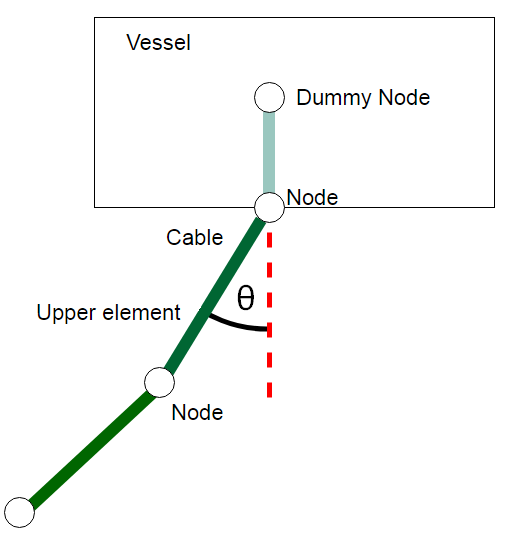
\includegraphics[scale=0.55]{figures/angle}
\caption[Angle between vessel and cable ]{Angle between vessel and cable  }
 \label{fig:angle}
\end{figure}

\noindent The angle was stored as a time series for each sea state. It was decided that the angle would be the master over the tension, meaning that for the local analyses, the cycle count for the angle would be used with the corresponding tension found by linear regression. \todo{skriv om regression her}

\begin{figure}[H]
\centering
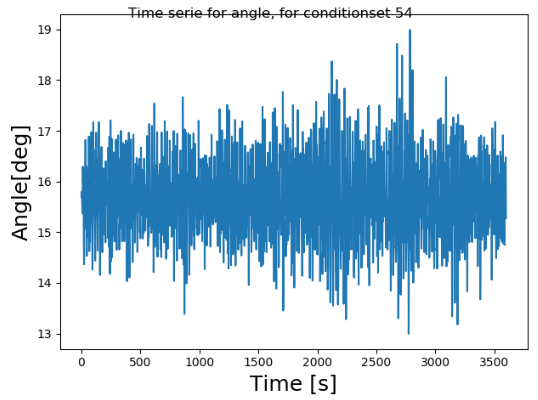
\includegraphics[scale=0.8]{figures/angtsex}
\caption[Example of a time series for Angle between vessel and cable  ]{Example of a time series for angle between vessel and cable}
 \label{fig:angleex}
\end{figure}

\subsection{Rainflow Counting}
As the angle was the master over the tension, Rainflow Counting was used on the time series of the angle to determine the number of cycles for each angle interval. The Rainflow Counting was performed in Python, and the algorithm is explained in Section \ref{sec:rainflow}. The Rainflow counting in Python gives a matrix where the first column is the angle interval and the second is the number of cycles in each interval. The counts from each sea state was normalized to apply for a year according to:

\begin{equation}
    n_{cycle,year}=n_{cycle,hour} \frac{n_{seastate}}{N_{seastate}} \cdot 365 \cdot 24 
\end{equation}

\noindent Where $n_{cycle,year}$ is the number of cycles of in an angle interval in a whole year, $n_{cycle,hour}$ is the number of cycles in an angle interval for an hour, calculated by the global analyses, $n_{seastate}$ is the number of observations of a certain sea state according to the scatter diagram in Figure \ref{fig:scatn} and $N_{seastate}$ is the total number of sea states in the scatter diagram in Figure \ref{fig:scatn}.\newline
\newline 
\noindent The results from the Rainflow Counting can be seen in Figure \ref{fig:ncyc}.  

\begin{figure}[H]
\centering
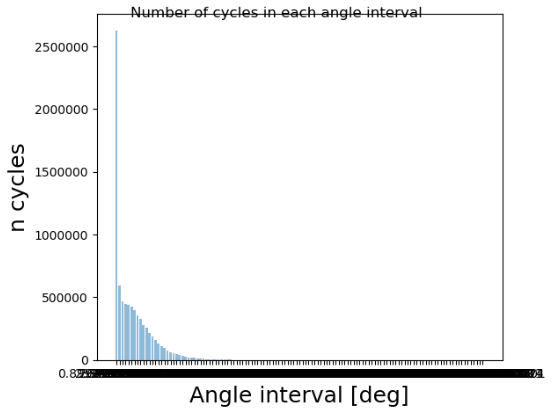
\includegraphics[scale=0.8]{figures/ncyc}
\caption[Number of cycles in each interval]{Number of cycles in each interval}
 \label{fig:ncyc}
\end{figure}

\noindent In Figure \ref{fig:ncyc}, the intervals are of equal length of 0.3. It is not possible to see the intervals on the x-axis due to the large amount of intervals. It is is clear from Figure \ref{fig:ncyc} that the majority of the cycles are happening in the first intervals, and decreasing as the angle increases.\newline
\newline
The damage from each cycle was calculated according to Miner Palmgren expression in Equation \ref{eq:MP}, where N was calculated from Equation \ref{eq:sn}. This gave the following expression for the damage from each angel interval: 
\begin{equation}
    d_i  = \frac{n_i}{N_i}
\end{equation}
Where $d_i$ is the damage from the cycles in angel interval i, $n_i$ is the number of cycles in angle interval i, $N_i$ is the number of cycles until failure for angle interval i.
\begin{equation}
    d_i=\frac{n_i}{\frac{c}{\Delta \sigma ^m}}
\end{equation}
Where $d_i$ is the damage from the cycles in angel interval i, $n_i$ is the number of cycles in angle interval i, c is a constant from Equation \ref{eq:sn}, c=4 for this case, $\Delta \sigma$ is the stress range that relates to the angle range as: $\Delta \sigma_i = a \Delta \theta_i$ where a is an arbitrary constant.\newline
\newline 
The damage from the cycles in the different angle intervals can be seen in Figure \ref{fig:di}

\begin{figure}[H]
\centering
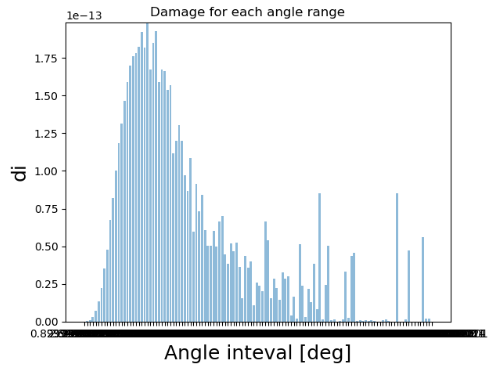
\includegraphics[scale=0.8]{figures/di}
\caption[Damage for each angle interval]{Damage for each angle interval}
 \label{fig:di}
\end{figure}
\noindent In order to get good results for the local analysis, the intervals need to be rearranges so that the damage is approximately the same over each interval. The results of this rearrangement can be seen in Figure \ref{fig:dire}

\begin{figure}[H]
\centering
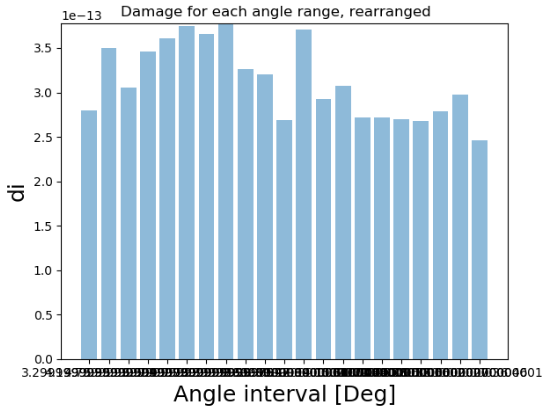
\includegraphics[scale=0.8]{figures/dire}
\caption[Damage for each angle interval, rearranged]{Damage for each angle interval, rearranged}
 \label{fig:dire}
\end{figure}

The rearrangement of the intervals led to the following interval and cycle distribution:

\begin{table} [H]
\centering
\begin{tabular}{ |c|c|}
\hline
Angle range [deg] & Number of cycles \\
 \hline
 \hline
0.0 - 3.3 & 6616323.9\\

3.4 - 4.2 & 559450.3\\
 
4.3 - 4.8 & 242007.9 \\
 
4.9 - 5.4& 170973.4  \\

5.5 - 6.0& 116753.1  \\

6.1  - 6.6 & 81592.7  \\

6.7 - 7.2 & 56956.2 \\

7.3 - 7.8 & 37457.6 \\

7.9 - 8.4 & 27639.9 \\

8.5 - 9.0 & 19444.0 \\

9.1 - 9.6 & 13779.9 \\

9.7 - 10.5 & 17029.9 \\

10.6 - 11.4 & 7031.5 \\

11.5 - 12.6 & 5340.2 \\

12.7 - 14.1 & 3213.0 \\

14.2 - 15.6 & 1830.2 \\

15.7 - 17.7 & 1227.9 \\

17.8 - 20.4 & 694.2 \\

20.5 - 24.3 & 351.7 \\

24.4 - 28.5 & 206.2 \\

28.6 - 36.6 & 89.9 \\

 \hline
\end{tabular}
\caption{Dimensions of local model}
\label{table:dim}
\end{table} 


\section{Local Analysis}
